\documentclass[journal]{IEEEtran}
% IEEE Transactions on Industrial Informatics -- anonymous regular-paper draft
% Compile: latexmk -pdf main.tex
\usepackage{amsmath,amssymb,amsfonts}
\usepackage{algpseudocode}
% Local XeTeX/Tectonic builds: route IEEEtran's ptm (Times) family requests to
% the legacy Times Type1 faces so metrics match the pdfLaTeX reference build;
% the latexmk -pdf (pdfLaTeX) path is unaffected.
\usepackage{iftex}
\ifxetex
  \DeclareFontFamily{TU}{ptm}{}
  \DeclareFontShape{TU}{ptm}{m}{n}{<->ptmr8t}{}
  \DeclareFontShape{TU}{ptm}{b}{n}{<->ptmb8t}{}
  \DeclareFontShape{TU}{ptm}{m}{it}{<->ptmri8t}{}
  \DeclareFontShape{TU}{ptm}{b}{it}{<->ptmbi8t}{}
  \DeclareFontShape{TU}{ptm}{m}{sl}{<->ptmro8t}{}
  \DeclareFontShape{TU}{ptm}{m}{sc}{<->ptmr8t}{}
\fi
\usepackage{graphicx}
\usepackage{booktabs}
\usepackage{tabularx}
\usepackage{array}
\usepackage[table]{xcolor}
\usepackage{stfloats}
\usepackage{placeins}
\usepackage{url}
% Allow line breaks at any character inside URLs/DOIs so long reference links
% do not leave ragged gaps at column edges (IEEE reference layout).
\usepackage{xurl}
\usepackage{etoolbox}
\urlstyle{same}
% Cross-references and citations. The cite package renders IEEE-style citation
% groups ([14]--[16], [20], [21]) with hyperref support.
\usepackage{cite}
\usepackage[colorlinks=true,linkcolor=black,citecolor=black,urlcolor=black]{hyperref}
\hypersetup{bookmarksnumbered=true,
  pdftitle={Agent-Mediated Online Data Acquisition and Governed Setpoint Control in Industrial Production Lines},
  pdfauthor={},
  pdfsubject={IEEE Transactions on Industrial Informatics},
  pdfkeywords={industrial agents, online data acquisition, agent-mediated control, governed setpoint control, industrial communication}}

% Float placement only; IEEEtran margins and body type remain unchanged.
\setcounter{topnumber}{4}
\setcounter{bottomnumber}{3}
\setcounter{totalnumber}{7}
\setcounter{dbltopnumber}{1}
\renewcommand{\topfraction}{0.95}
\renewcommand{\bottomfraction}{0.80}
\renewcommand{\textfraction}{0.03}
\renewcommand{\floatpagefraction}{0.72}
\renewcommand{\dbltopfraction}{0.95}
\renewcommand{\dblfloatpagefraction}{0.72}

% Tight but conventional float separation; body type and margins are unchanged.
\setlength{\textfloatsep}{8pt plus 2pt minus 3pt}
\setlength{\dbltextfloatsep}{8pt plus 2pt minus 3pt}
\setlength{\intextsep}{7pt plus 2pt minus 3pt}
\setlength{\abovecaptionskip}{3pt plus 1pt minus 1pt}
\setlength{\belowcaptionskip}{2pt plus 1pt minus 1pt}

\newcommand{\system}{the platform}

\begin{document}
\bstctlcite{IEEEbstctl}

\title{Agent-Mediated Online Data Acquisition and Governed Setpoint Control in Industrial Production Lines}

\author{}
\markboth{IEEE Transactions on Industrial Informatics, Submitted Manuscript}{Agent-Mediated Setpoint Control}

\maketitle

\begin{abstract}
Industrial agents that acquire process data and propose setpoint changes require a runtime that relates equipment operations to production context and controls access to them. This article presents a configuration-driven runtime for agent-mediated data acquisition and governed setpoint control. A production scene binds line, product, recipe, and run context to distinct acquisition and control mappings and registered protocol drivers. Agent harnesses provide acquisition and control-intent tools, while task-mediated and direct calls enter a shared dispatcher. The runtime applies applicable authorization and configured write limits, with route-specific revalidation following approval when required; command outcomes, optional readbacks, and later process observations remain distinct. In direct-interface probes of 55 write-capable endpoints across four simulated scenes and five protocols, all 220 admissible requests received the expected acceptance response and all 219 collected out-of-range requests received the expected rejection. In an exploratory simulator comparison, a bounded scripted policy had lower retained-window integrated absolute error than a no-write condition in all nine selected scene--seed blocks; the batch-selection rule remains unresolved. Three language-model-driven injection episodes were canceled below target. These results characterize selected application-level behaviors, while a complete correlated agent-to-device trace and physical-plant performance remain unverified.
\end{abstract}

\begin{IEEEkeywords}
Industrial agents, online data acquisition, agent-mediated control, governed setpoint writing, industrial communication, simulation-based evaluation.
\end{IEEEkeywords}

\IEEEpeerreviewmaketitle

\section{Introduction}
\IEEEPARstart{P}{roduction-line} integration for an industrial agent couples online data acquisition with governed control. The agent acquires process observations and production context, relates them to an objective, and proposes a typed setpoint or recipe adjustment. The runtime resolves the relevant line, process variable, and control signal before applying authority and limits. For example, a cast-film line-speed setpoint may affect measured film thickness, but the control and acquisition nodes remain distinct even when both use Message Queuing Telemetry Transport (MQTT). Acquired observations, command acceptance, device readback, and later process measurements are separate evidence. Fig.~\ref{fig:control-path} illustrates this distinction.

Research on industrial agents includes service supervision and skill-based manufacturing \cite{biskupovic2025supervision,koehle2026llmdriven}. Other studies examine semantic grounding, approval, and verification for plant-facing operations, including programmable logic controller (PLC) interfaces \cite{graul2026aas,schall2026safe}. Fault-recovery planning is another area of study \cite{vyas2026detection}. These studies leave unresolved how a runtime should connect an agent's online acquisition and analysis to a controlled operation across task-mediated and direct entry paths. This paper examines that boundary without claiming a new control law or agent-reasoning algorithm.

We enforce five invariants: observations inform an agent proposal but do not grant write authority; acquisition and control mappings are direction-specific; an approved control intent is revalidated; command receipts, readbacks, and later process observations remain separate; and task-mediated and direct calls converge on one guarded boundary. A scene binds line, product, recipe, and run to mappings, drivers, objectives, and limits. Direct API and fixture tests assess selected paths; a complete correlated agent-to-device trace would require retained harness, acquisition, driver, readback, and observation records.

The contributions are:
\begin{enumerate}
  \item A production-scene model linking context, direction-specific acquisition/control mappings, registered drivers, objectives, and limits for agent-facing operations. (Section~III.)
  \item An agent-to-operation boundary in which registered harnesses acquire observations and submit control intents, while direct callers use the same dispatch, revalidation, approval, and write guards. (Sections~III--V.)
  \item An evidence-bounded evaluation of acquisition/control mappings and governance responses, supplemented by an exploratory simulator comparison and language-model-driven episodes. (Section~VI.)
\end{enumerate}

\begin{figure}[!b]
\centering
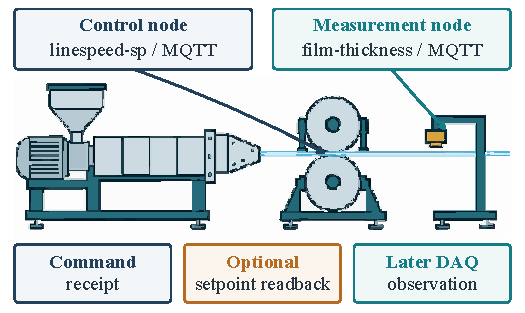
\includegraphics[width=0.98\columnwidth]{resources/fig1-vectorized-20261109.pdf}
\caption{Illustrative configured cast-film example: an agent acquires film-thickness data and may propose a line-speed adjustment, but the line-speed control node and film-thickness acquisition node remain distinct even though both use MQTT. Command acceptance or optional setpoint readback is distinct from the later process observation.}
\label{fig:control-path}
\end{figure}



\section{Related Work}
\label{sec:related}
Table~\ref{tab:related-comparison} summarizes the selected systems discussed below. Their different tasks, interfaces, and evaluation units allow a qualitative comparison, not a ranking or head-to-head benchmark.

\begin{table*}[!t]
\centering
\caption{Representative related work and the scope of its reported evaluation. The studies address different tasks and are not a common benchmark. OPC UA: Open Platform Communications Unified Architecture.}
\label{tab:related-comparison}
\footnotesize
\setlength{\tabcolsep}{5pt}
\begin{tabularx}{\textwidth}{@{}>{\raggedright\arraybackslash}p{0.16\textwidth}>{\raggedright\arraybackslash}p{0.40\textwidth}X@{}}
\toprule
Study & Main focus & Reported setting \\
\midrule
Biskupovic et al.~\cite{biskupovic2025supervision} & Agent-based industrial service selection and reselection & Service adaptability and performance in an industrial cyber--physical system \\
K\"{o}hle et al.~\cite{koehle2026llmdriven} & Module-specific agents and skill-based manufacturing & Nine simulated production challenges \\
Graul et al.~\cite{graul2026aas} & Grounded proposals, documented authorization, and proposed PLC-side checks & Two proof-of-concept scenarios using a simulated OPC UA server \\
Schall~\cite{schall2026safe} & Process-diagram, supervisory control and data acquisition (SCADA), and procedure-grounded verification & Five simulated scenarios and proposal evaluation \\
Vyas et al.~\cite{vyas2026detection} & Multi-agent fault-recovery planning with a process-plant twin & Simulated mixing and stirred-tank reactor studies \\
This work & Scene-bound signal mappings, shared dispatch, and route-specific governance & Simulator and mock-driver probes, scripted missions, and exploratory live-Agent episodes \\
\bottomrule
\end{tabularx}
\end{table*}

\subsection{Industrial Agents and Plant Integration}
Biskupovic et al. study online service selection and reselection in industrial cyber--physical systems \cite{biskupovic2025supervision}. Xia et al. present a digital-twin-connected automation architecture and control generation \cite{xia2025architecture,xia2025control}; other work generates PLC programs \cite{liu2026agents4plc}. In related control research, human instructions have also been incorporated into model-predictive control \cite{wu2025instructmpc}.

Li et al. use structured instructions, retrieval, and iterative verification to generate and check finite-element scripts for Abaqus; that study evaluates engineering-artifact generation rather than runtime authority over process writes \cite{li2026modsolagent}. Other studies examine large language model (LLM) agents, manufacturing skills, and natural-language machine interaction \cite{koehle2026llmdriven,lim2025llmenabled,zhao2026shopfloor,hofmann2025nlc}. Vyas et al. combine multi-agent fault-recovery planning and plant-knowledge retrieval with Digital Process Plant Twin studies of mixing and continuous stirred-tank reactors (CSTRs) \cite{vyas2026detection}.

These studies address agent organization, generated actions, or task execution. The present study does not introduce an agent policy or control law. It examines the runtime boundary that carries production context and direction-specific signal mappings into an operation and applies the required checks before dispatch.

\subsection{Industrial Interfaces and Semantic Commissioning}
Agent-facing interface work includes Model Context Protocol (MCP) access to manufacturing resources \cite{silva2025mcpmanufacturing}, semantic recipes built from Open Platform Communications Unified Architecture (OPC UA) skills \cite{koehle2025semanticrecipes}, industrial-protocol adapters \cite{xavier2026industriConnect}, and tools for binding manufacturing data to a cognitive digital twin \cite{liu2026semanticcommissioning}. These systems address capability discovery, protocol access, or commissioning. Here, configuration binds known protocol drivers to scene-specific read and write nodes. A named operation resolves those bindings through a runtime path that checks authority and write limits. We do not treat MCP or a semantic node name as an authorization mechanism.

\subsection{Governed Operations and Verification}
Prior work also examines plant-facing verification. Graul et al. propose grounding plans in the Asset Administration Shell, with documented human authorization and PLC-side validation of OPC UA Methods \cite{graul2026aas}. Schall verifies proposals against piping and instrumentation diagrams, SCADA data, and standard operating procedures; Lin and Chen describe a policy-governed sensor--manufacturing execution system (MES)--enterprise resource planning (ERP) digital thread \cite{schall2026safe,lin2026agentic}. PLCBench evaluates autonomous agents against commercial PLCs with hardware-in-the-loop process simulation \cite{zhou2026plcbench}. These studies complement the runtime examined here and illustrate established concerns about authorization and safety controls. Our implementation examines how configured signal bindings, route-specific checks, shared dispatch, and separate command and process records operate together at the write boundary. This is a system-integration contribution; the studies use different settings and do not establish comparative safety.

\subsection{Production Context and Outcome Evidence}
MCP standardizes tool discovery and invocation \cite{mcp2026}. For industrial operations, application-layer services must still enforce operation-specific authority and process constraints. ISA-88 and ISA-95 define recipe and production-operation concepts \cite{isa88_2010,isa95_2025}. Run-to-run control relates process observations to subsequent decisions, while human--automation research examines allocation of responsibilities between people and automation \cite{moyne2001r2r,parasuraman2000model}. These studies establish important pieces of industrial-agent integration, but they do not make the boundary invariants used here explicit as one operation contract. In particular, the literature does not jointly expose context as non-authorizing information, direction-specific acquisition/control bindings, post-approval route revalidation, typed separation of command/readback/process evidence, and convergence of task-mediated and direct calls on the same guarded boundary. The present work therefore makes these invariants explicit and evaluates selected application-level admission paths in simulators and mock-driver fixtures. This is a system-integration contribution, not a claim of comparative control efficacy, functional safety, or complete agent-to-device provenance.

\section{System Design}
\label{sec:design}
The runtime exposes named services through two entry paths. Task-mediated calls use the collaboration runtime and a registered agent harness; the harness gives the agent scoped tools for online acquisition, analysis, and control-intent submission. Direct REST or stdio-MCP calls provide verification and integration paths. Both enter the shared dispatcher, while scene configuration supplies context, acquisition bindings, objectives, and write limits.

\begin{figure*}[!t]
\centering
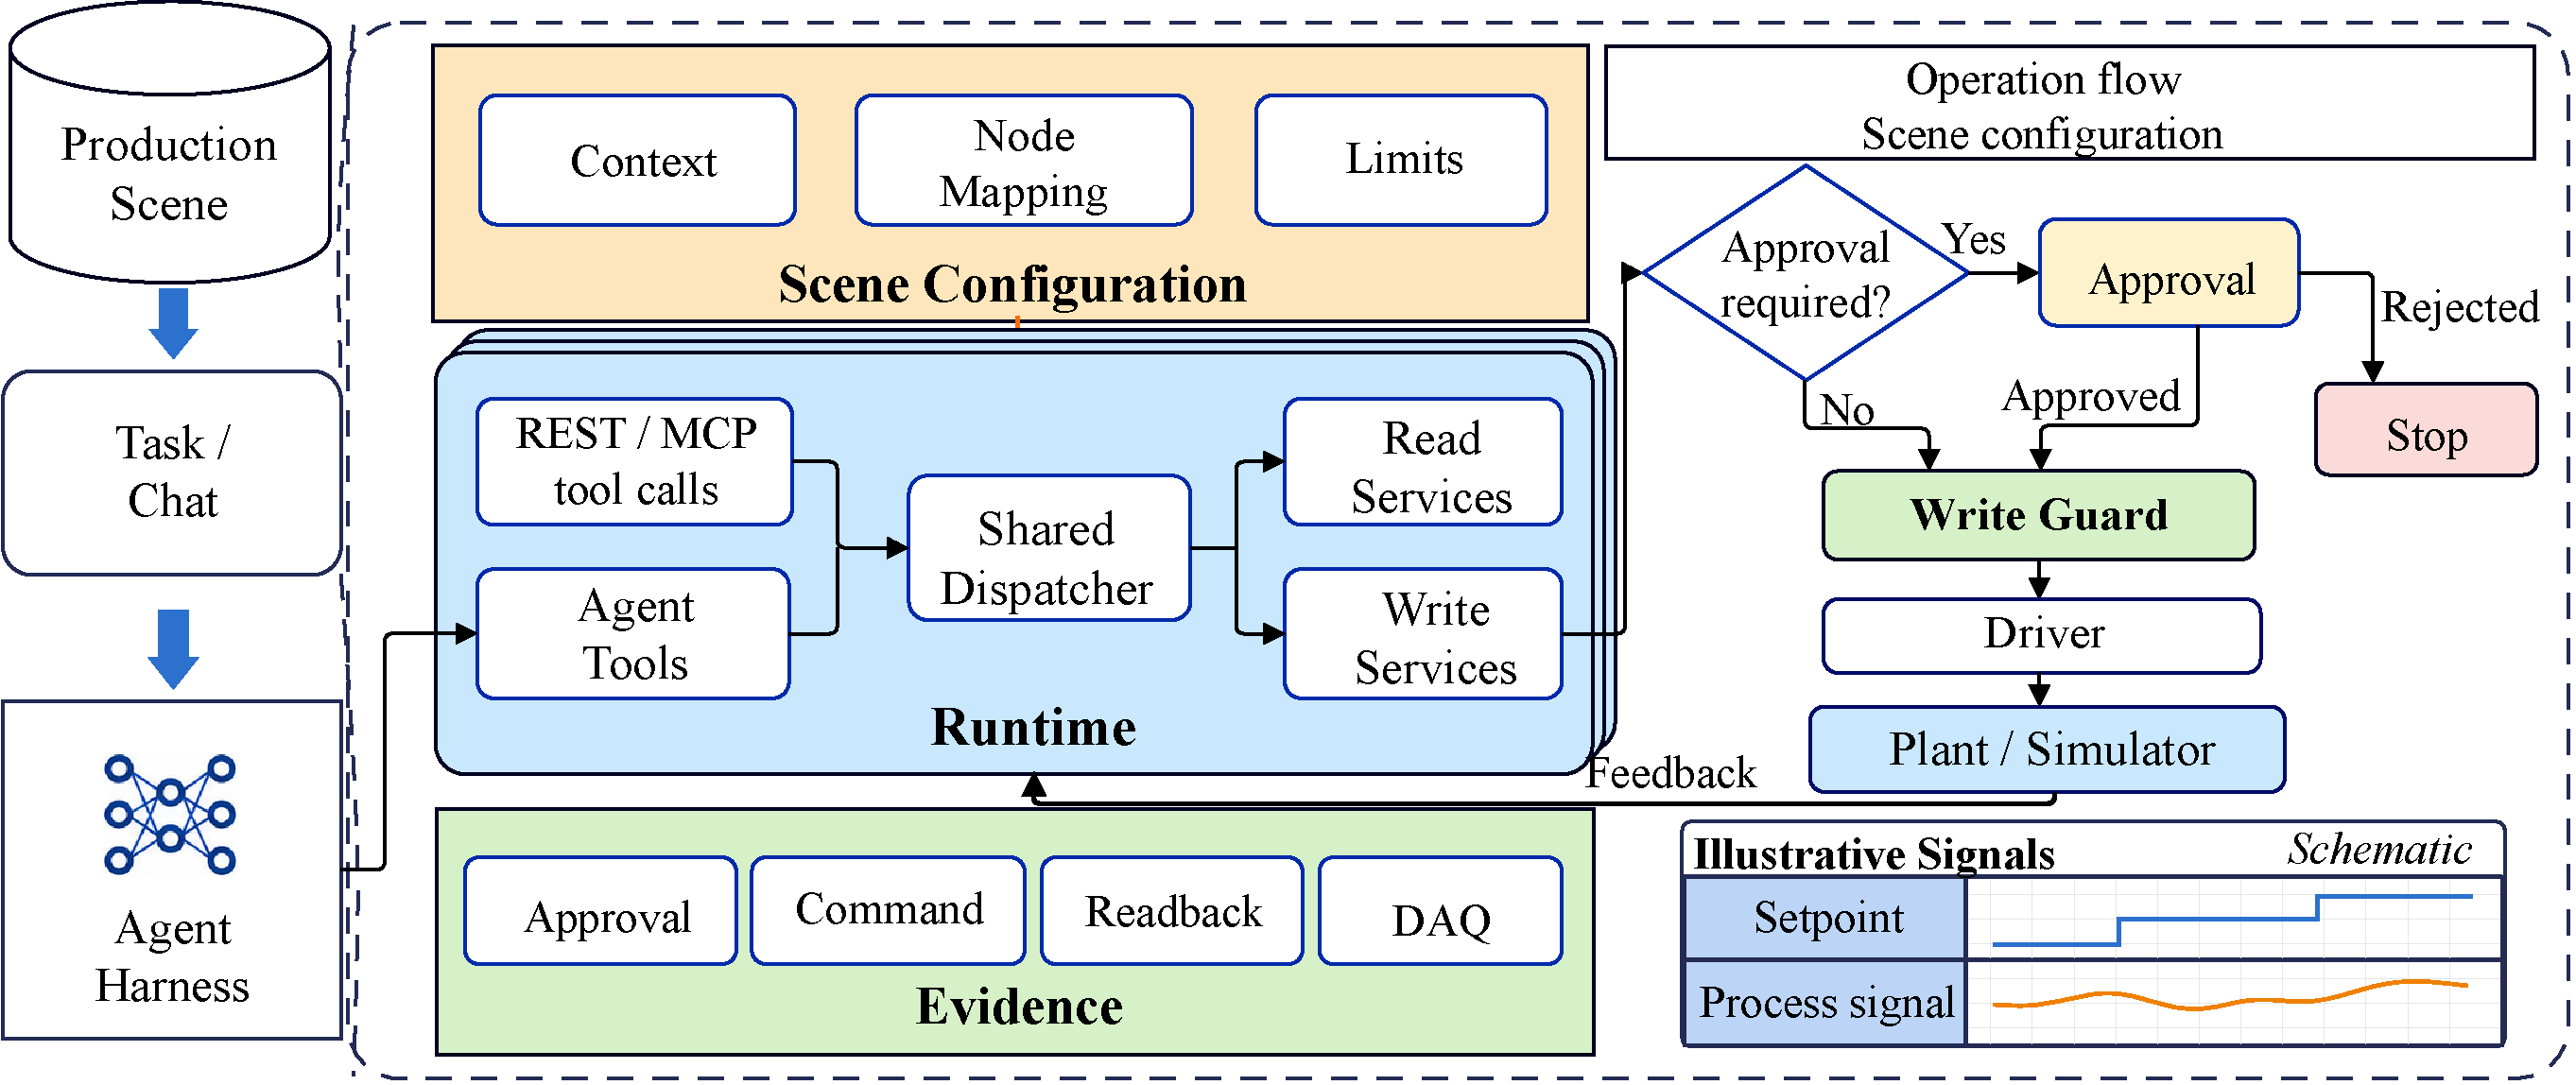
\includegraphics[width=\textwidth]{resources/fig2.pdf}
\caption{Task-mediated and direct tool calls share a dispatcher; a registered agent can acquire observations and submit a control intent, while direct calls provide a verification path. Direct calls need no task. Approved intents undergo route-specific revalidation (omitted here; see Fig.~\ref{fig:hitl}). The no-approval path remains subject to applicable authorization and write guards. Requests rejected by pre-dispatch checks stop before driver dispatch. Feedback and signals are schematic, not measured traces. Approvals, command outcomes, optional readbacks, and later data-acquisition (DAQ) observations are distinct records. In-flight exclusion rejects overlapping writes per node and process; equipment interlocks remain necessary.}
\label{fig:arch}
\end{figure*}

\subsection{Design Rationale and Requirements}
\label{sec:principles}
The runtime must preserve process meaning across heterogeneous drivers, provide a stable contract for registered harness adapters, and check authority and process limits before each control write. It distinguishes acquired process data from command acceptance and later observations. Scene configuration, registered adapters, shared dispatch, route handlers, and service-owned records enforce these boundaries.

The context builder assembles production context and eligible observations for an agent turn. The agent uses them to form a proposal, but context and observations do not grant write authority; the handler resolves live state when the control operation is invoked.

\subsection{Layered Architecture}
\label{sec:layers}
Fig.~\ref{fig:arch} shows the system layers. Task and chat routes use registered harness adapters that provide scoped acquisition and control tools; binding and channel policy constrain available operations. Agent analysis remains distinct from deterministic boundary checks. The figure also shows a schematic feedback path and illustrative signals.

Direct REST agent-tool calls and the stdio-MCP bridge bypass task execution and enter the shared dispatcher. The task route gives the agent context, acquisition targets, and objectives; operation services resolve control mappings and guards. Read/analysis services (DAQ, MES access, retrieval, and optional model services) are separated from write and recipe services. Input/output mappings connect semantic nodes to built-in or plugin drivers, and owning services retain task, command, observation, and configuration records.

\subsection{Scene Configuration as the Integration Boundary}
\label{sec:scene-config}
Scene-specific process semantics are configured before
they are used by an operation. The active line identifies the production context; product
and recipe records supply applicable targets and limits; the run record
provides the current operating state. Semantic nodes bind process variables
to direction-specific acquisition or control mappings, and the driver
registry resolves each mapping to a supported protocol implementation. Here
\emph{semantic} denotes a named process variable with a direction, unit, and
configured mapping; it is not an OPC UA or Asset Administration Shell
information model. Each agent-facing operation is named and typed, so a harness need not
construct protocol-specific messages. A scene using an already registered
driver can supply different context and node mappings behind the same
operation contract. A protocol not present in the registry still requires a
driver adapter; configuration alone does not implement a new protocol.

In the cast-film simulator preset, for example, the MQTT command mapping
\texttt{linespeed-sp} controls line speed in m/min, while the distinct
\texttt{film-thickness} mapping supplies thickness in $\mu$m. An agent can
acquire the thickness observation, compare it with its objective, and propose a
line-speed intent; the runtime admits that intent against the control node's
limits. Sharing MQTT does not make either signal a substitute for the other.

Table~\ref{tab:scene-config} summarizes how the execution path uses the scene
description and distinguishes configuration-time bindings from checks against
live state. The context assembled for an agent turn describes the active scene. Before a
write, the handler resolves the live state required by its route and applies
the current limits. Where a route supports context snapshots, approval is
bound to both the proposal and the context. The command receipt remains
separate from subsequent DAQ observations.

\begin{table*}[!t]
\centering
\caption{Scene configuration elements and their roles in the runtime path.}
\label{tab:scene-config}
\footnotesize
\setlength{\tabcolsep}{5pt}
\begin{tabularx}{\textwidth}{@{}>{\raggedright\arraybackslash}p{0.19\textwidth}>{\raggedright\arraybackslash}p{0.34\textwidth}X@{}}
\toprule
Element & Configured information & Runtime use\\
\midrule
Production context & Line, product, recipe, and run associations & Context construction for a task turn; route-dependent live-state checks before a write\\
Semantic I/O & Process variable, direction, unit, and node mapping & Acquisition uses the read mapping; accepted operations resolve the configured control mapping\\
Driver binding & Supported protocol driver and endpoint configuration & Driver registry selects the protocol implementation after operation checks\\
Operation admission & Engineering, baseline, product, and recipe limits; step and timing rules where configured & Route handler checks the candidate against current bounds and rejects inadmissible requests\\
Approval policy & Whether approval is required and the decision validity window & Pending request binds the proposed action; route-specific checks run after approval\\
Evidence ownership & Command receipt, verification grade, and later DAQ observations & Owning services retain command outcomes separately from process measurements\\
\bottomrule
\end{tabularx}
\end{table*}

\subsection{Cross-Module Execution Flow}
\label{sec:executionflow}
For a task-mediated call, the registered adapter presents a scoped tool
catalog containing acquisition, context, and control operations to the agent.
The agent reads available observations, relates them to the task objective, and
submits a typed intent rather than a protocol-specific message. At the
operation boundary, the shared dispatcher checks the predicates declared for
the named operation before selecting its handler. The handler resolves live
production state, applies route-specific guards and limits, and requests any
required approval before device I/O.

For an industrial operation $u$ by agent $a$ in channel $c$, define the
shared dispatch condition as
\begin{equation}
\mathcal{A}(a,c,u)=\bigwedge_{X\in\mathcal{C}(u)}X(a,c,u).
\label{eq:dispatch-contract}
\end{equation}
In Eq.~(\ref{eq:dispatch-contract}), $S$, $P$, $G$, and $B$ denote invocation scope, current channel policy,
applicable industrial grant, and the agent's binding to referenced resources,
respectively. $\mathcal{C}(u)\subseteq\{S,P,G,B\}$ is the set of predicates
declared for operation $u$; it always contains $S$ and $P$. The grant predicate
$G$ is included when the resolved channel, target line, and owner/grant policy
require it; explicit exemptions omit it. The binding predicate $B$ is included
when the operation declares resource references. An operation that declares
no references omits $B$. Each included check must pass before handler
selection. The policy predicate includes channel tool selection, profile, and duty-separation checks where
configured.

Once these predicates pass, the selected route applies its operational
guards and requests any required approval. For example, an exploration request checks
the control binding and DAQ visibility before entering the governed write
path; an invisible target returns an error before a write. The checks performed
after approval depend on the route; Section~\ref{sec:modules} specifies the
single-node and recipe-operation paths.

For a direct REST agent-tool call, the service establishes $a$ and $c$ before applying
these checks. An agent token must match the requested agent identifier; an
authenticated user must be the channel owner or an administrator. The manager
loads the channel-agent record and rechecks scope and policy, followed by any
applicable grant and binding checks. Handlers resolve live production state
using request identifiers and the owning services.



\section{Agent-Coordinated Task-Level Operation}
\label{sec:closed-loop-operation}

\begin{figure*}[!t]
\centering
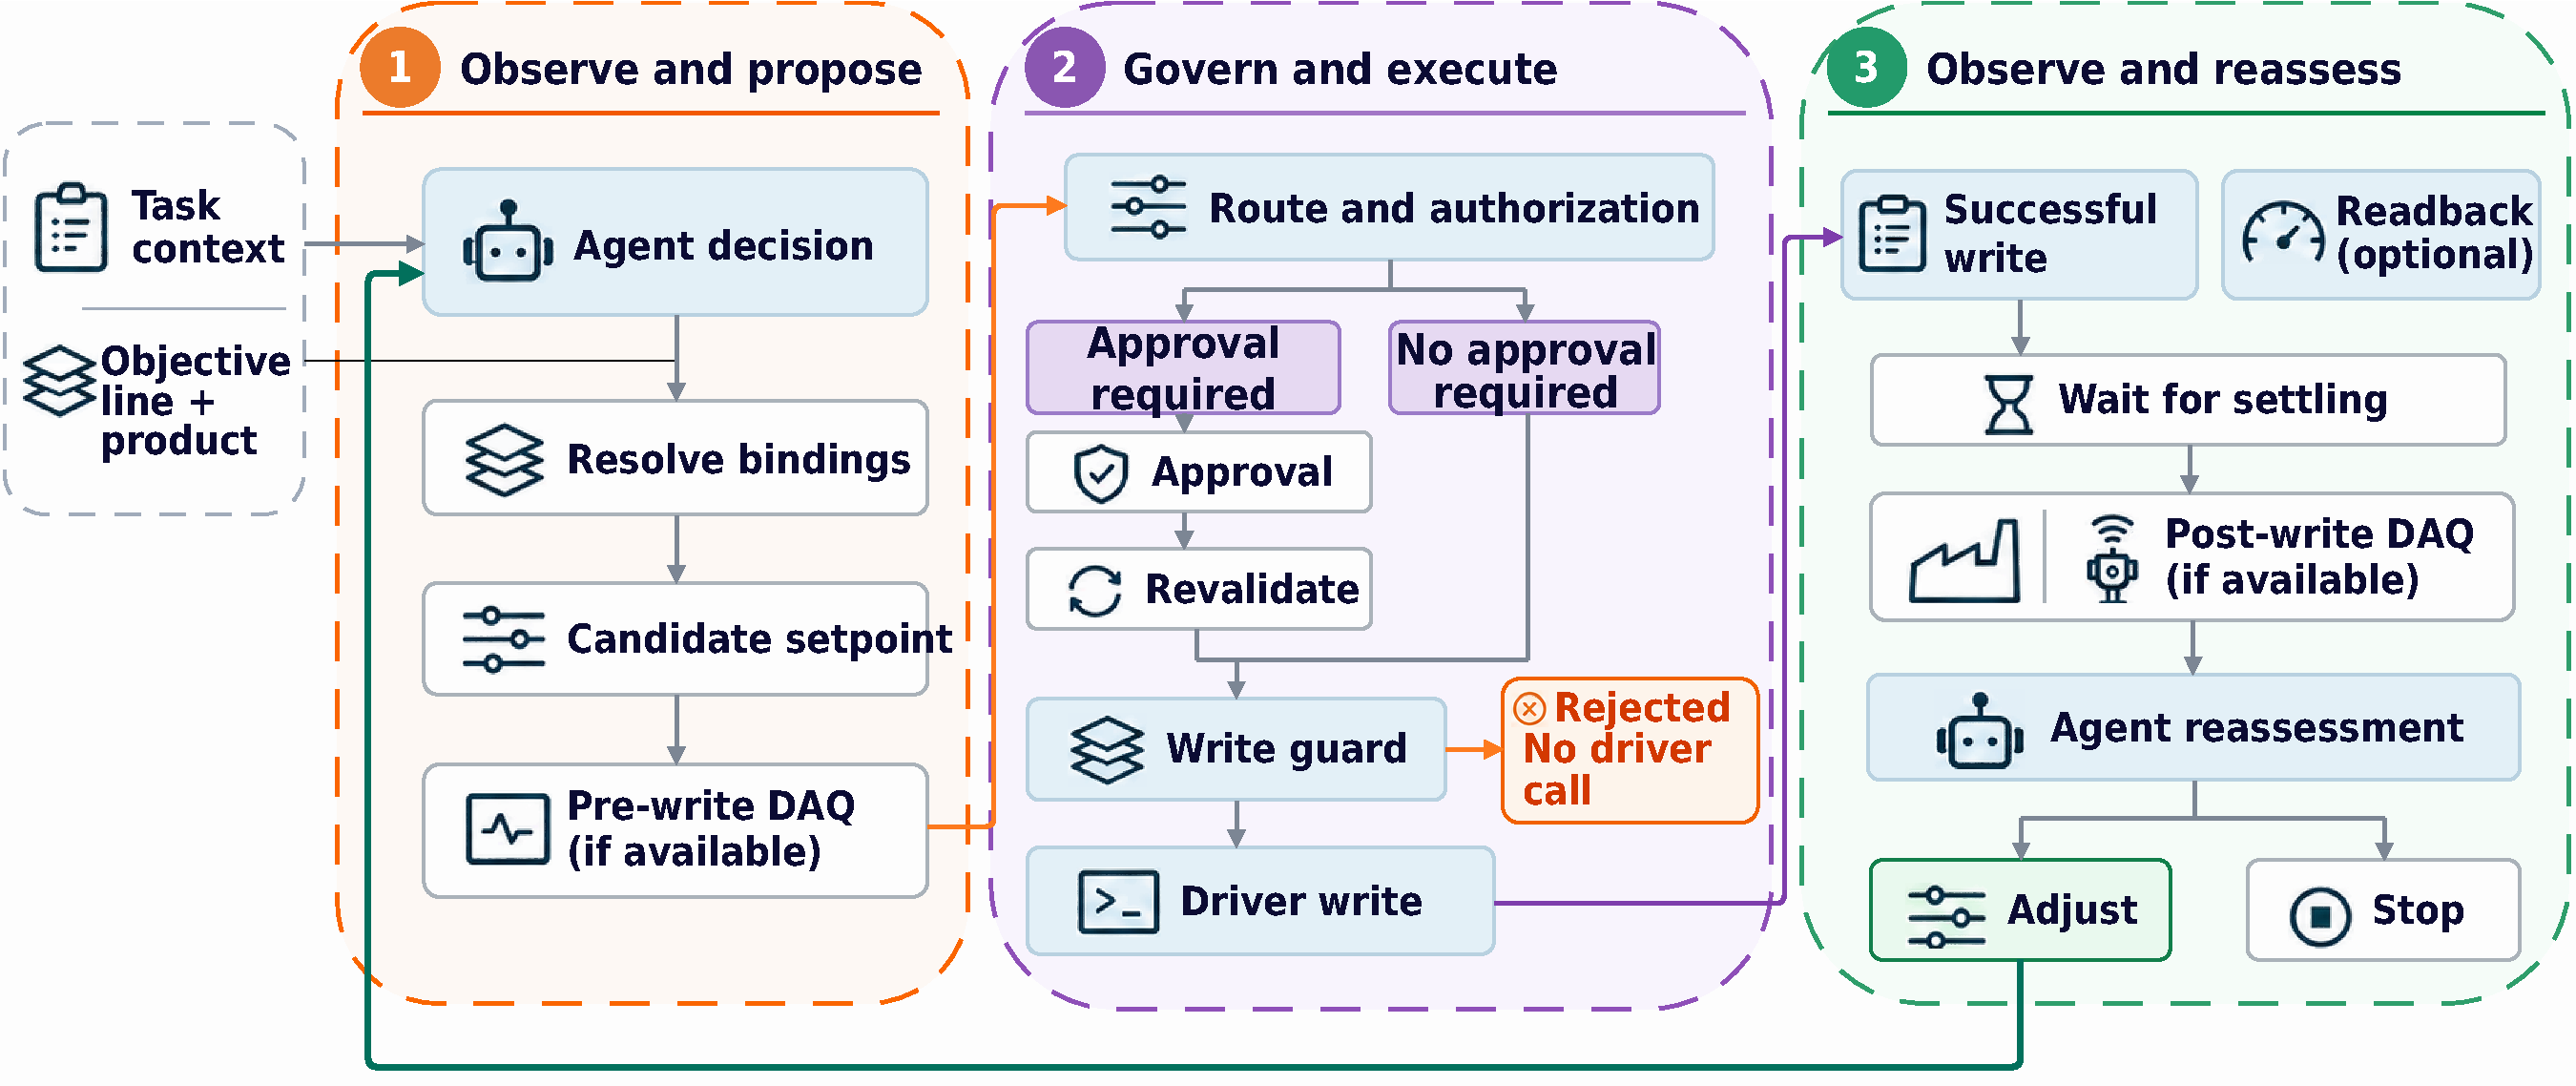
\includegraphics[width=\textwidth]{resources/fig3.pdf}
\caption{Conceptual agent-mediated online acquisition and control loop: the agent acquires observations, analyzes the objective gap, proposes a setpoint, and the write path applies route-dependent checks before controlled dispatch. The agent may reassess returned evidence before another adjustment or stopping. Requests requiring approval proceed to route-specific revalidation only after approval; requests denied before dispatch do not reach the driver. The approval-denial branch is omitted. Routes without required approval bypass the approval wait but remain subject to applicable dispatch, authorization, and write-guard checks. A driver error may leave device state uncertain. Command outcomes and optional readback are distinct from later DAQ observations; the readback box is schematic.}
\label{fig:agent-loop}
\end{figure*}

A task supplies an objective and production context. In the intended workflow, the agent acquires configured DAQ or read-only observations, analyzes them, and proposes a typed adjustment. Fig.~\ref{fig:agent-loop} traces this conceptual iteration through governed execution and reassessment; it does not depict a successful live-Agent run. Data and context inform but do not authorize a write. The control node comes from \texttt{control\_node\_id} or a configured binding; the DAQ target comes from an explicit ID or agent DAQ binding.

In goal mode, a lead agent may decompose the objective and dispatch worker subtasks. For each step, the responsible agent invokes \texttt{optimization\_explore}, which acquires the DAQ target, checks bindings, and submits a candidate before device I/O.

The operation resolves the profile and control binding, then reads the stored value as $u_0$; this is not necessarily a fresh readback. The agent combines this state with its objective and direction. If direction is omitted, the operation defaults upward; otherwise $s\in\{-1,+1\}$. For a step $\Delta u$, it forms
\begin{equation}
 u^{*}=\operatorname{clip}\!\left(u_0+s\Delta u,\,u_{\min},\,u_{\max}\right).
 \label{eq:optimization-candidate}
\end{equation}
In Eq.~(\ref{eq:optimization-candidate}), configured tuning bounds take precedence; node bounds are used otherwise. The effective step is selected in this order: an explicit argument, the binding's tuning step, the scene's maximum step, or one twentieth of the node range.

The operation resolves the DAQ target and checks visibility before the intent enters the governed path. Later implementation gates include identifiability and model--ontology checks; these were added after the reported experiments. If the checks pass, the operation attempts a pre-write DAQ read, whose mean may be unavailable.

A valid candidate enters the governed single-node write path in Algorithm~1. A pre-dispatch denial stops the request before a driver call. A driver-stage error may occur after dispatch begins, so status alone cannot establish whether the device changed; state must be read and reconciled before retrying.

After a successful write, the operation returns the command outcome and supported readback to the agent, waits 10--300~s (45~s by default), and attempts a post-write DAQ read. Later windows are $[t_0-\tau,t_0]$ and $[t_0,t_1]$; approval may include pre-dispatch samples, so the mean is not causal. The earlier implementation reads trailing 45-s windows.

The exploration record returns the target, step, available DAQ means, and write status/message; the shared path separately records command outcome and readback. On a later turn, the agent can inspect returned evidence, choose another step, or stop; iteration requires a subsequent agent decision.



\section{Operation Governance and Evidence}
\label{sec:modules}
Section~\ref{sec:design} defines the shared dispatch contract. This section
focuses on the checks that follow an agent's control intent: scene-specific write admission,
conditional approval, and the records returned by each route.

\subsection{Scene-Specific Write Admission}
\label{sec:governed}
Authorization and value admission are checked separately. The target band describes a desired
process outcome; it does not define the admissible write interval. A candidate may
satisfy all write constraints even when the measured process value remains outside
the target band.

For an online node write, the admissible value interval is
\begin{equation}
\mathcal{I}^{\mathrm{online}}_n(t)=
\mathcal{H}_n\cap\mathcal{L}^{\mathrm{base}}_n\cap\mathcal{L}^{\mathrm{prod}}_n(t)\cap\mathcal{L}^{\mathrm{rec}}_n(t),
\label{eq:admission}
\end{equation}
where $\mathcal{H}_n$ is the hard engineering range, and
$\mathcal{L}^{\mathrm{base}}_n$, $\mathcal{L}^{\mathrm{prod}}_n$, and
$\mathcal{L}^{\mathrm{rec}}_n$ are the baseline, active-product, and
active-recipe limits. These numerical bounds are distinct from the scope,
policy, grant, and binding predicates in Eq.~(\ref{eq:dispatch-contract}).
An absent optional limit imposes no restriction; an empty intersection admits no
candidate. The controller checks each candidate against the configured layers
and identifies the first violated layer when a limit is exceeded. Recipe dispatch
checks a replacement recipe against the hard, baseline, and product limits,
rather than the previous recipe's window. Trial overrides are additionally checked against
the applicable recipe window.

Algorithm~1 summarizes how an agent or direct caller's single-node control intent is admitted after shared dispatch. For
\texttt{optimization\_explore}, it shows the ordinary full-limit profile; a failed
check stops the request before driver dispatch. A benchmark ablation can
omit soft limits while retaining the hard engineering range.

\par\medskip
\noindent\begin{minipage}{\columnwidth}
\small
\noindent\textbf{Algorithm 1:} Governed online single-node write
\par\kern2pt\hrule\kern2pt
\begin{algorithmic}[1]
\Require Node $n$, candidate $x$, and channel if present
\Ensure Rejection or driver outcome and available readback
\State Check execution mode, value, and node authorization
\If{approval is required}
  \State Request a decision for $(n,x)$ and wait
  \If{decision is declined or expires}
    \State \Return rejection
  \EndIf
  \State Revalidate the original authorization path
\EndIf
\State Recheck the grant if a channel is present
\State Check gateway/node state and controller guards
\State Resolve $\mathcal{I}^{\mathrm{online}}_n$; reject if $x\notin\mathcal{I}^{\mathrm{online}}_n$
\If{not benchmark mode}
  \State Check step, interval, and hold window
\EndIf
\State Dispatch $x$ to the configured driver for $n$
\State \Return outcome and available readback
\end{algorithmic}
\kern2pt\hrule
\end{minipage}
\par\medskip

The operation uses an agent control-intent source; recipe and rollback sources follow
their own paths. A driver-stage error may leave device state uncertain.
These application-level
checks complement, but do not replace, equipment interlocks.

\subsection{Approval, Execution, and Evidence}
\label{sec:mech}

\begin{figure*}[t]
\centering
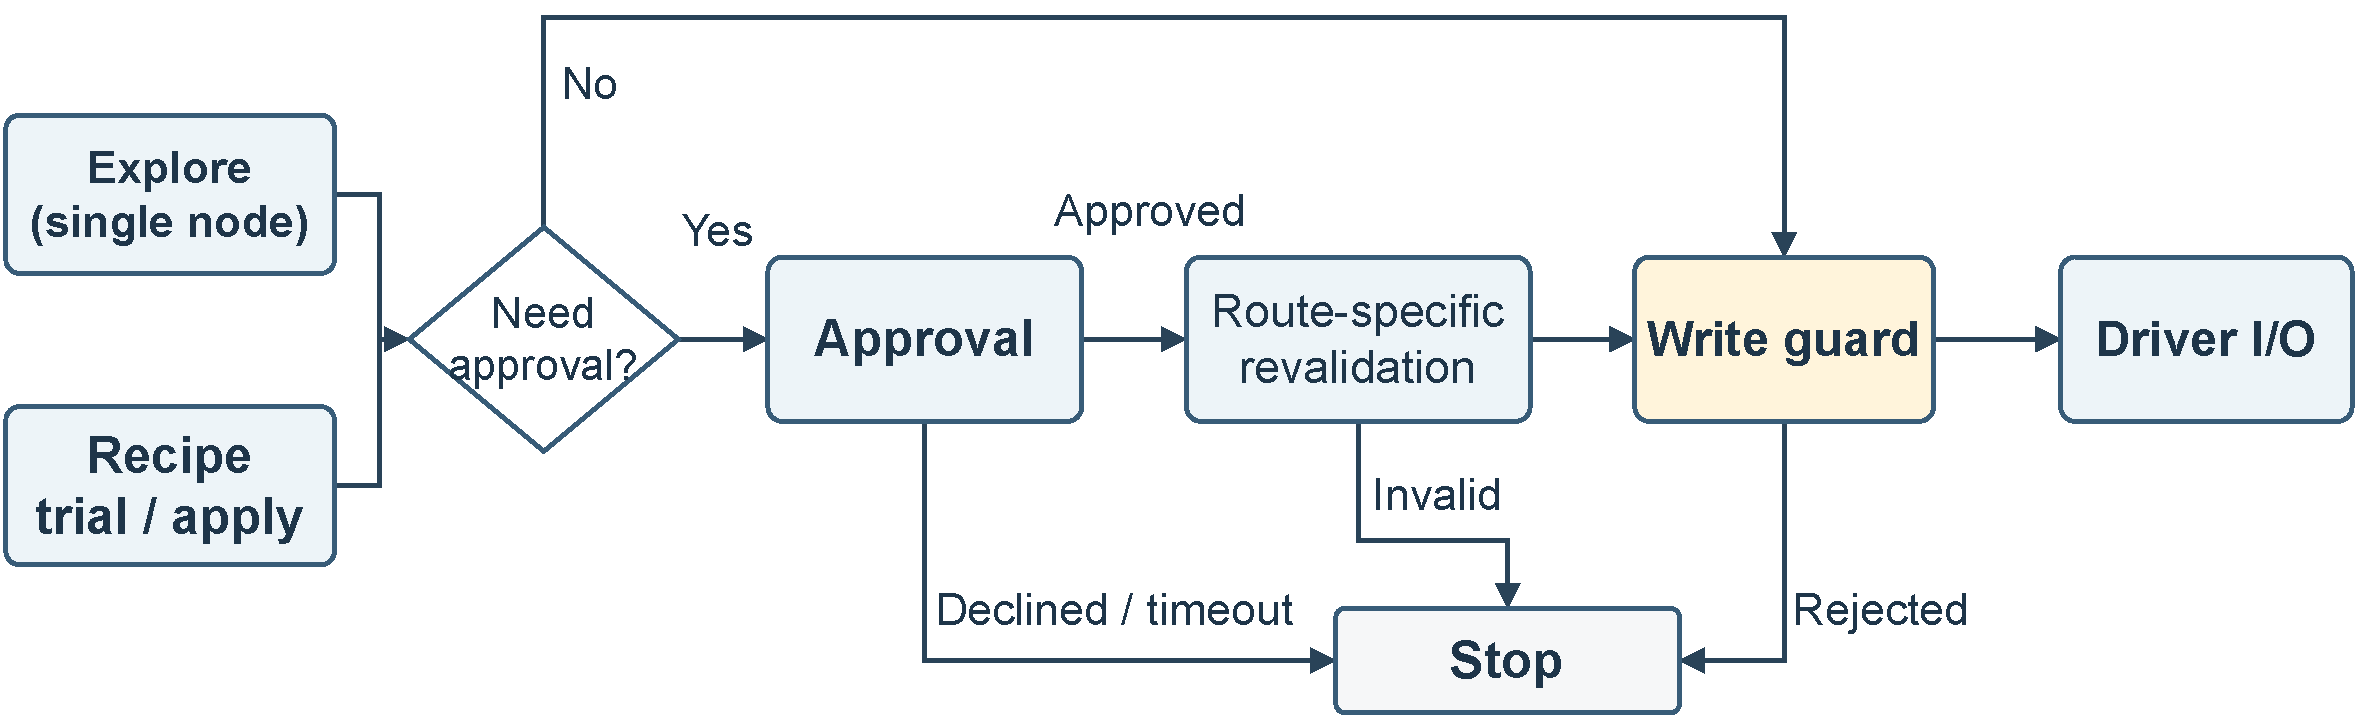
\includegraphics[width=\textwidth]{resources/fig4-governed-flow.pdf}
\caption{Simplified single-node \texttt{optimization\_explore} and recipe trial or apply write paths. Approved requests undergo route-specific revalidation. A decline, timeout, failed revalidation, or guard rejection stops the affected operation or parameter before driver dispatch. Other applicable dispatch and authorization checks are omitted; bypassing approval does not bypass them.}
\label{fig:hitl}
\end{figure*}
Fig.~\ref{fig:hitl} shows the conditional approval path from an agent or manual control intent and the bypass to the shared write guard. For a manual single-node \texttt{optimization\_explore}
request, the approval service receives the node, proposed value, current
effective interval, and rationale. The same governed boundary receives an agent's typed intent after its acquisition and analysis step. As in Algorithm~1, a decline or timeout
stops the request, while approval triggers revalidation of the original
direct node binding or the recipe binding and parameter membership. This path
does not use the recipe-operation context snapshot described below.
Revalidation does not make the checks and external device write atomic.

Recipe operations use a separate approval path. For \texttt{recipe\_trial}
and \texttt{recipe\_apply}, the approval is bound to the recipe operation and
active line--product--recipe--run context. After approval, the handler checks
authority and context again and verifies the recipe definition and
candidate scope before dispatch. A changed context, revoked binding, or
changed recipe definition prevents that proposal from proceeding. Recipe
trial approvals use a 30-minute window by default; single-node approval waits
expire after 180\,s by default. Outside benchmark mode, agent and manual
writes are subject to a minimum 60-s interval following a setpoint change;
recipe trials also use a per-line cadence of 300\,s by default.

A \texttt{recipe\_trial} submits a bounded batch from the agent's control intent through the configured
driver and returns a result for each parameter to the calling route. Parameters are attempted
individually, so a batch can be partially applied; results and device state
must be reconciled before the agent or caller retries. A trial does not save or apply a recipe
version. Before updating, applying, or rolling back the recipe, the caller can
retrieve later DAQ observations separately.

Receipts record the command outcome returned to the agent or caller; observations record what followed in
the process. Command results are graded as readback-verified,
transport-acknowledged, or unverified. When a successful recipe write is not
already readback-verified, the service may, by default, attempt up to three additional
reads at 2\,s intervals where supported; recipe batches retain verification
outcomes for each parameter. A readback-verified result means that the
returned value matched the request within the applicable tolerance. A transport
acknowledgement alone does not establish that the device applied the value, and
an unverified result does not establish a matching readback. DAQ stores later
timestamped process observations for the agent's next analysis turn, while
recipe history, approvals, and task records remain with their owning services.
Identifiers and timestamps can link these records when available, but a later
observation alone does not prove that the command caused the measured change.
Section~\ref{sec:eval} evaluates selected parts of this evidence chain under the
stated test conditions.



\section{Experimental Evaluation}
\label{sec:eval}
The evaluation examines three evidence layers of an agent-mediated operation path: configured acquisition and control mappings, application-level governance routes, and subsequent process observations. The intended agent workflow acquires configured observations, analyzes them against a process objective, and submits a control intent to the shared dispatcher. We first test the mappings and limits through selected direct API requests, then report an exploratory simulator contrast between a scripted policy representing bounded control-intent execution and a no-write condition. Separate fixtures examine guard and approval-route responses. An injection-twin run and three LLM-driven episodes are non-evaluative follow-up observations rather than complete agent-to-device trials; the episodes ran on the \texttt{omp} agent-harness engine with a DeepSeek Flash (\texttt{deepseek-flash}) model endpoint.

Integrated checks used already-running platform and simulator services, generally in benchmark mode, which bypasses step, interval, and hold-window checks for agent or manual writes. Individual ablation configurations also removed selected checks. No cold-start deployment or physical-plant run was performed.

A service response, a simulated readback, and a later process measurement are distinct. An acquired observation supports the agent's analysis but does not grant authority; an accepted control intent does not by itself establish driver dispatch, and a later process value does not identify the write that caused it.

\subsection{Configured Mapping and Integration Checks}
\label{sec:eval-mapping}
Two integrated executions, both with seed~42, each passed 77 assertions across 17 phases. Both began with the platform and simulator already running, and neither activated an agent harness. A film-line preset check configured five endpoint types and rejected nine selected negative probes; it reused the same runtime and is not an independent deployment replication. These runs therefore assess the acquisition/control mapping and direct runtime/API behavior used by the agent-facing boundary, not a complete task-mediated agent path.

The scene--protocol probes covered 55 configured write-capable endpoints in four simulated scenes using Modbus Transmission Control Protocol (TCP), Modbus remote terminal unit (RTU), OPC Unified Architecture (OPC UA), Message Queuing Telemetry Transport (MQTT), and Hypertext Transfer Protocol (HTTP). Table~\ref{tab:scene-probe-results} gives the scene-level counts. The probe plan specified three requests for interior values, one for the upper boundary, and four for values outside the structural range at each endpoint. All 220 requests with prespecified admissible values received the expected acceptance response; all 219 collected out-of-range requests received the expected rejection, and all 216 available simulator readbacks matched. These probes assess selected mappings; the tested values and guards derive from the same configured limits. One structural request was not collected; HTTP endpoints do not expose readback, and the scene--protocol matrix is incomplete.

\begin{table*}[!t]
\centering
\caption{Configured scene--protocol probes. Counts show prespecified admissible requests receiving the expected acceptance response, out-of-range requests receiving the expected rejection, and matching simulator readbacks where supported.}
\label{tab:scene-probe-results}
\footnotesize
\setlength{\tabcolsep}{3pt}
\begin{tabularx}{\textwidth}{@{}>{\raggedright\arraybackslash}p{1.55cm}r X r r r@{}}
\toprule
Scene & Configured endpoints & Protocols represented & Accepted probes & Structural rejects & Simulator readbacks \\
\midrule
Injection & 11 & TCP 5; RTU 2; OPC UA 3; MQTT 1 & 44/44 & 44/44 & 44/44 \\
Wastewater & 7 & TCP 1; RTU 3; OPC UA 2; MQTT 1 & 28/28 & 28/28 & 28/28 \\
Annealing & 7 & TCP 3; RTU 2; OPC UA 1; MQTT 1 & 28/28 & 28/28 & 28/28 \\
Biaxial line & 30 & TCP 20; RTU 1; OPC UA 8; HTTP 1 & 120/120 & 119/119 & 116/116 \\
\bottomrule
\end{tabularx}
\end{table*}

\subsection{Exploratory Fixed-Horizon Simulator Contrast}
\label{sec:eval-optimization}
We compared a deterministic bounded setpoint policy with a no-write condition in injection, wastewater, and annealing simulations. The policy used the \texttt{recipe\_trial} route. The available candidate policy adjusts injection holding pressure and time, wastewater blower and dosing settings, and annealing-zone temperatures and line speed according to scene-specific conditions. The target bands were $32.5\pm0.35$~g for part weight, $3.4\pm0.6$~mg/L for dissolved oxygen, and $95\pm6$~HV for hardness, respectively. Each scene used its own fixed horizon (180~s for injection; 240~s for the other scenes), nominal one-second sampling, an independent reset for each arm, and a pre-specified initial-process-value window. Arm order was randomized within each scene--seed block, but paired starts were not required to have identical process values. The primary outcome was integrated absolute error (IAE), the time integral of the absolute deviation from the target, calculated by the trapezoidal rule over the retained samples between the first and last retained points. Internal gaps up to 5~s were linearly interpolated; no extrapolation was made to the nominal window endpoints, and a larger gap invalidated the pair.

In the later batch of 11 post-pilot scene--seed blocks, nine met the reset, initial-window, and sampling rules. Two blocks (wastewater seed~45 and annealing seed~46) were invalid because their no-write traces had 9-s and 6-s gaps. An earlier batch also contains an independently reset, valid injection seed-44 block with $\Delta\mathrm{IAE}=193.320$~g\,s; the later batch repeated that block and yielded 165.165~g\,s. The available records do not establish a batch-selection rule, and the earlier batch contains failed reset attempts; the reported subset is therefore exploratory. Every valid block in the later batch had a positive $\Delta\mathrm{IAE}=\mathrm{IAE}_{\mathrm{no\text{-}write}}-\mathrm{IAE}_{\mathrm{scripted}}$. Among the valid blocks, recorded samples from every scripted run entered its target band, whereas none from the no-write runs did. Table~\ref{tab:selected-iae} reports per-scene medians and ranges; the complete selected-batch records, invalid blocks, earlier block, and exclusion rationale are provided in Supplementary File~S7 and the accompanying evidence archive.

\begin{table}[!t]
\centering
\caption{Selected fixed-horizon simulator contrasts. Positive $\Delta$IAE means lower retained-window accumulated absolute error under the scripted policy.}
\label{tab:selected-iae}
\footnotesize
\setlength{\tabcolsep}{3pt}
\begin{tabular}{@{}lcc@{}}
\toprule
Scene (unit of $\Delta$IAE) & Valid & Median (range) \\
\midrule
Injection (g\,s) & 3/3 & 165.165 (162.535--195.169) \\
Wastewater ((mg/L)\,s) & 3/4 & 615.605 (611.670--630.980) \\
Annealing (HV\,s) & 3/4 & 8000.450 (7930.200--8084.150) \\
\bottomrule
\end{tabular}
\end{table}

The unresolved batch-selection rule limits inference from these results. The sample is small, simulator seeds are not independent plants, and no proportional--integral--derivative or model-predictive-control baseline was tested. The run record reports a combined SHA-256 matching local copies of the paired-run and scene-policy scripts. This self-reported hash does not independently establish the executed process image, and a complete service and simulator snapshot was not identified. The archive therefore does not support full end-to-end reproduction. Accordingly, we make no significance or broad efficacy claim.

Fig.~\ref{fig:optimization-trajectory}(a) shows the mass traces for the three valid injection blocks, and Fig.~\ref{fig:optimization-trajectory}(b) tabulates their recorded setpoint requests. For each scripted mass trace, a recorded sample entered the target band within the first 15~s; subsequent samples fluctuated near its lower boundary, whereas the no-write traces stayed near their initial values. The task logs report a 31.2~g baseline, which need not equal the first sample in the plotted horizon. Seeds~44 and~45 each recorded a pressure request followed by a hold-time request; seed~46 recorded a further pressure request (58$\rightarrow$61.88~bar) after its hold-time request. The task script's final post-settling means were 32.163, 32.190, and 32.383~g, respectively, within the 32.15--32.85~g band. The starting and requested values in Fig.~\ref{fig:optimization-trajectory}(b) are script records, not independent device readbacks. For seed~46, a prior request to 57.97~bar and a later recorded starting value of 58~bar are shown as recorded. The archive neither aligns requests with acquisition timestamps nor preserves a per-request server ledger. Fig.~\ref{fig:optimization-trajectory}(c)--(e) compare IAE for the nine selected blocks by scene; Table~\ref{tab:selected-iae} reports the contrasts.

\begin{figure*}[!t]
\centering
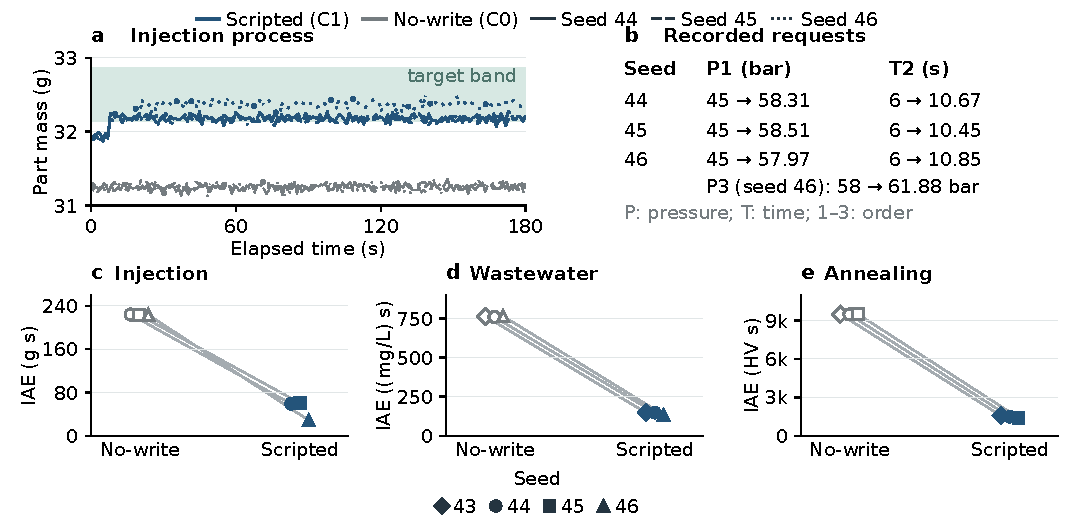
\includegraphics[width=\textwidth]{resources/fig5.pdf}
\caption{Selected simulator observations. (a) Recorded part-mass samples for the three valid injection scene--seed blocks over the nominal 180~s window; the shaded band is 32.15--32.85~g. Color distinguishes no-write (C0) from the scripted policy (C1), and line style identifies the seed. Sampling gaps beyond 1.5~s appear as breaks and isolated samples as dots; no smoothing is applied. (b) Recorded starting and requested setpoints: P and T denote hold pressure and hold time, and subscripts give request order, not timestamps. These are script records, not independent simulator-device readbacks. (c)--(e) Retained-window IAE for the nine selected scene--seed blocks; markers identify seeds. Each line connects one contrast, and small horizontal offsets only separate overlapping markers. Each scene uses its own scale and native unit multiplied by seconds, so magnitudes are not comparable across scenes. The two blocks invalidated by sampling gaps and the earlier repeated injection block are excluded; the selection rule is unresolved.}
\label{fig:optimization-trajectory}
\end{figure*}

\subsection{Write-Guard and Route Behavior}
\label{sec:eval-ablation}
The process-window guard-path comparison used direct API requests in one simulated scene with a mock driver. These requests represent control intents at the shared operation boundary, not complete agent episodes. Four configurations retained or removed the process-window and readback checks; hard structural limits remained active. Each configuration was tested in three repetitions, each using four structural violations, two process-window violations, three legal values, and three boundary values; the specific violation values differed across configurations. Additional timed writes in each repetition were excluded from these counts. Each configuration rejected all 12 structural violations and falsely blocked none of its nine legal requests. The full-guard and no-readback configurations rejected all six window violations (HTTP~400; shown as 6/0 rejected/accepted in Fig.~\ref{fig:guard-approval-results}(a)). The configurations without the process-window check, with or without the readback check, accepted all six window violations (HTTP~200; 0/6 rejected in each configuration). Each configuration met all 9/9 boundary expectations defined for it: outside-window values were expected to be accepted when the window check was removed. These repeated fixture responses are not independent trials. The archive contains no per-request driver-call ledger, and the comparison did not stimulate a readback mismatch; readback-guard effects are therefore not assessed by this fixture. Fig.~\ref{fig:guard-approval-results}(a) shows the recorded responses by configuration and request class.

In a separate follow-up batch, all 110 tested values outside configured recipe windows but within structural limits were rejected. In a simulated readback-fault probe, a 230-unit command returned 251 against a 0.7-unit tolerance and was marked \texttt{unverified}; one baseline and one recovery call were marked \texttt{readback-verified}. Production-mode branch checks rejected one case each for interval, step, node range, recipe window, and hold window, and accepted a legal baseline. Separate authorization checks rejected an unbound request and a cross-node request and accepted a bound write. These fixtures characterize the selected branches and inputs, not physical-device safety.

The approval-route pilot used four scripted calls with simulated setpoints. With the approval route enabled, an approved call changed 202 to 204.8, whereas a rejected call left 216 unchanged. Two bypass-route calls changed 202 to 204.8 and 216 to 218.8. The automatic-arm labels do not match the starting values of their purported approval-arm counterparts. Consequently, these four cases illustrate route behavior but do not constitute a clean matched approval ablation; a scripted proxy, not an operator, supplied the approval decisions. Fig.~\ref{fig:guard-approval-results}(b) plots the recorded before and after values for each call.

\begin{figure*}[!t]
\centering
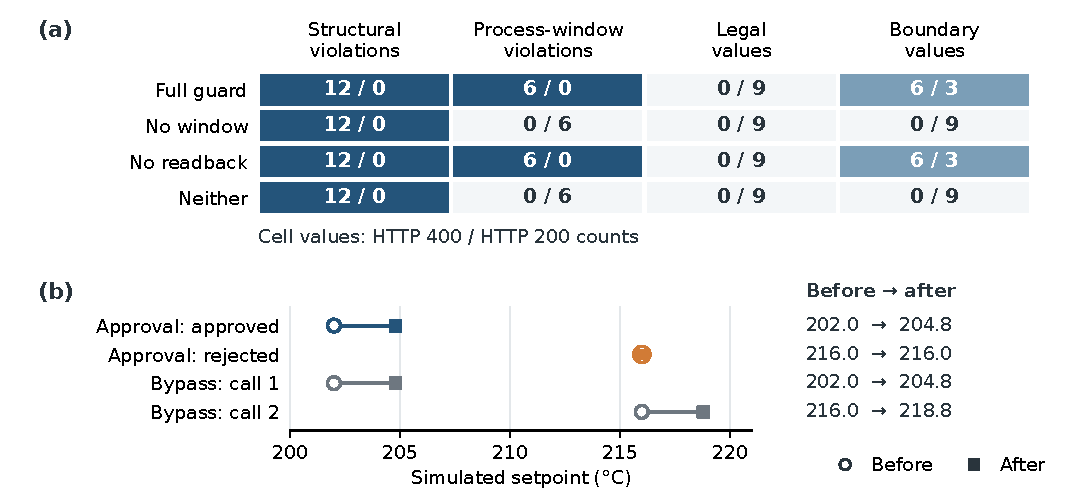
\includegraphics[width=\textwidth]{resources/fig6.pdf}
\caption{Guard-path comparison and scripted approval-route results. (a) Counts of HTTP~400 and HTTP~200 responses for four guard configurations and four request classes, with three repetitions per configuration. Each cell lists rejected/accepted counts, and their sum is the class total; shading represents the proportion of HTTP~400 responses. The specific violation values and boundary expectations differed across configurations. The comparison did not stimulate a readback mismatch. (b) Recorded before and after simulated setpoints for four separate calls; open circles mark before and filled squares after. A scripted proxy supplied the approval decisions, and the bypass calls required no approval. The calls are not matched pairs. HTTP~200 does not establish driver dispatch.}
\label{fig:guard-approval-results}
\end{figure*}

\subsection{Injection-Twin Demonstration}
\label{sec:eval-twin-pilot}
An acceptance script ran one experiment on a PLC-based simulated twin (\texttt{realPlant=false}). A governed write changed the setpoint from 60 to 63.7~bar, the simulated readback matched, and three later samples averaged 32.224~g after the specified wait. The structured baseline is 31.503~g, whereas the report states 31.508~g; the discrepancy and missing raw sample series and runtime snapshot prevent this run from supporting an effect estimate.

\subsection{LLM-Driven Simulator Episodes}
\label{sec:eval-agent}
Three LLM-driven injection episodes ran under the \texttt{omp} agent-harness engine with a DeepSeek Flash (\texttt{deepseek-flash}) model endpoint; the saved worker label is blinded and the served model snapshot identifier was not retained. All three episodes ended \texttt{CANCELED} below the 32.15--32.85~g band, at 31.70, 31.87, and 31.99~g. Each worker trace records one \texttt{recipe\_trial} call to update two setpoints and a response reporting both as acknowledged; approval was automatic, and one episode carries a guard-violation flag. The row-level server journal was not retained, so these responses do not independently verify driver dispatch. The episodes do not estimate agent success, operator approval effects, or physical execution.


\section{Discussion}
\label{sec:discussion}
The runtime makes the intended agent-mediated sequence explicit: the agent acquires configured process observations, analyzes them against an objective, submits a control intent, receives a command outcome or supported readback, and can request later DAQ observations for a subsequent decision. The selected nominal fixed-horizon batch had lower retained-window accumulated error with the deterministic policy than with no-write in all nine selected valid blocks. An earlier valid block was repeated in the selected batch, and the available records do not explain the batch-selection rule. There were only three selected blocks per scene. Initial process values were constrained to windows rather than required to match exactly, and no named conventional controller was tested. The result therefore supports a comparison specific to these simulations, not a claim of general process-control efficacy.

Fig.~\ref{fig:optimization-trajectory} presents the recorded injection mass traces and pressure and hold-time requests alongside the selected retained-window IAE contrasts. These records do not establish the causal effect of each setting: iteration-level timing and independent per-request server records are unavailable.

The mapping and guard tests support only the configured branches and inputs that were exercised. The test oracles share configuration with the tested limits, and the mock-driver ablation lacks independent dispatch records. Simulator readback is not physical actuation evidence. The LLM-driven episodes exercised the agent-facing recipe tool and returned acknowledged updates, but all ended below target. Without the server journal, those responses cannot establish a complete agent-to-device write chain. Agent task completion, command acknowledgement, and process attainment must therefore remain separate outcomes.

The platform and simulator were already running, and a complete immutable service and configuration snapshot was not retained. Application checks complement PLC, safety-instrumented-system, and equipment protections. Further process validation requires a larger pre-specified study with verified reset states, common sampling and horizons, a named controller baseline, and complete trajectories. Agent evaluation requires a fixed acquisition-and-control task, retained model and runtime versions, and correlated observation-to-intent-to-device records for every episode. Human-approval effects and physical safety need separate studies.

\section{Conclusion}
\label{sec:conclusion}
This work presents a configuration-driven runtime for agent-mediated online data acquisition and governed setpoint control. The agent-facing path binds production context and direction-specific acquisition/control signals, returns observations for objective-conditioned analysis, and carries a typed control intent through route-dependent checks before dispatch while keeping command outcomes distinct from readback and later process observations. Selected mapping and guard branches were exercised across simulated scenes and mock-driver fixtures. In the selected nominal fixed-horizon simulator batch, all nine valid scene--seed pairs had lower retained-window IAE under the deterministic setpoint policy than under no-write; an earlier valid pair was repeated and the batch-selection rule is unresolved. This exploratory result lacks a conventional controller baseline. The injection traces show recorded setpoint requests and process observations; three LLM-driven episodes exercised the agent-facing recipe tool but were canceled below target and lacked a complete server-side write record. The evidence establishes an application-level agent-to-operation integration boundary, not general optimizer convergence, autonomous-agent efficacy, a complete agent-to-device trace, or physical-plant safety.


\section*{Declarations}
The authors declare no competing interests. This anonymous study used simulated scenes, mock-driver fixtures, and a PLC-based simulated twin; no human participants, personal data, or physical-plant data were involved. Author contributions and funding are withheld during anonymous review and will be provided in the final version. Generative AI was used for limited language editing and source organization; the authors reviewed the manuscript and remain responsible for its technical content, results, and claims. The evidence is supplied in the anonymous supplementary package and supporting-evidence archive; no physical-plant data were collected.

\bibliographystyle{IEEEtran}
% \IEEEtriggeratref{10} removed 2026-11-13: with the longer data-availability
% statement the forced break spilled the remaining references onto an 11th
% page; natural flow ends on page 10.
\bibliography{resources/refs}

\end{document}

